\documentclass[a4paper,10pt]{article}
\usepackage{tikz}
\usepackage{verbatim}
\usepackage[margin=15mm]{geometry}
\usetikzlibrary{shapes,arrows,fit,calc,positioning}


\begin{document}

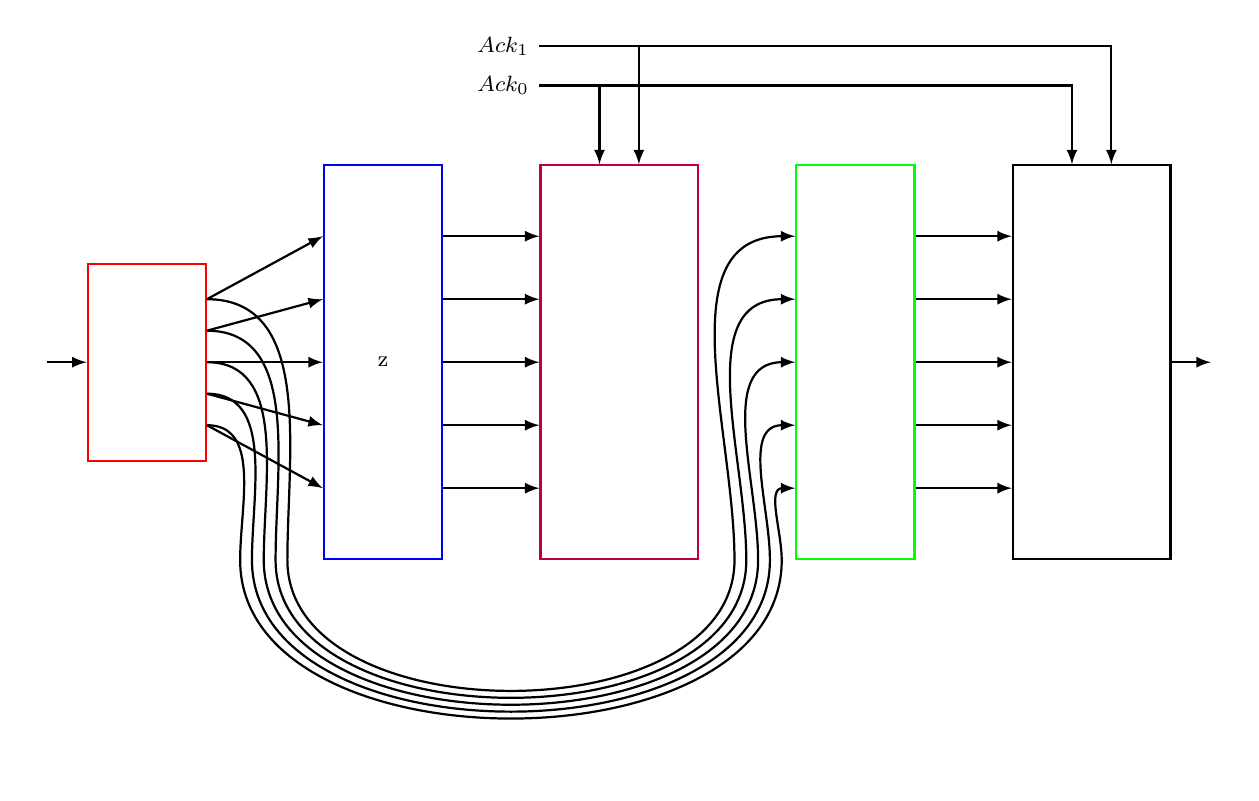
\begin{tikzpicture}[thick]
\tikzset{input/.style={}}
\tikzset{block/.style={rectangle,draw}}
\tikzstyle{pinstyle} = [pin edge={to-,thick,black}]

\node [input, name=input] {};
\node [block, right=0.5 cm of input,minimum width=1.5cm, minimum height=2.5cm,red] (a) {};
\node [block, right of=a,minimum width=1.5cm, minimum height=5cm,node distance=3cm,blue] (b) {};
\node [block, right of=b, minimum width=2cm, minimum height=5cm,node distance=3cm,purple] (c) {};
\node [block, right of=c,minimum width=1.5cm, minimum height=5cm,node distance=3cm,green] (d) {};
\node [block, right of=d, minimum width=2cm, minimum height=5cm,node distance=3cm] (e) {};
\node [right =0.5 cm of e] (output) {};

\begin{scope}[->,>=latex]

\draw[->] (input) -- (a);

\node at (b.center) {\footnotesize{z}};

\draw[->] ([yshift=1.5 cm]c.north west) node[left]{\footnotesize{$Ack_1$}} -| ([xshift=0.25 cm]e.north);
\draw[->] ([yshift=1.5 cm]c.north west) -| ([xshift=0.25 cm]c.north);
\draw[->] ([yshift=1 cm]c.north west) node[left]{\footnotesize{$Ack_0$}} -| ([xshift=-0.25 cm]e.north);
\draw[->] ([yshift=1 cm]c.north west) -| ([xshift=-0.25 cm]c.north);
\draw[->] (e) -- (output);

\foreach \i in {2,...,-2}{%
\draw[->] ([yshift=\i * 0.4 cm]a.east) -- ([yshift=\i * 0.8 cm]b.west) ;}

\foreach \i in {-2,...,2}{%
\draw[->] ([yshift=\i * 0.8 cm,]b.east) -- ([yshift=\i * 0.8 cm]c.west) ;}

\foreach \i in {-2,...,2}{%
\draw[->] ([yshift=\i * 0.4 cm]a.east) to [out=-0,in=90]  ([xshift={\i * 0.15 cm-0.75cm}]b.south west) to [out=-90,in=-90]  ([xshift={-\i * 0.15 cm+0.75cm}]c.south east)  to [out=90,in=-180]  ([yshift=\i * 0.8 cm]d.west) ;}

\foreach \i in {-2,...,2}{%
\draw[->] ([yshift=\i * 0.8 cm]d.east) -- ([yshift=\i * 0.8 cm]e.west) ;}

\end{scope}
\end{tikzpicture}



\begin{tikzpicture}
  \node[anchor=east] at (0,0) (text) {This is some text.};
  \node[anchor=west] at (3,1) (description) {Here is the description.};
  \draw (description) edge[out=180,in=0,->] (text);
\end{tikzpicture}

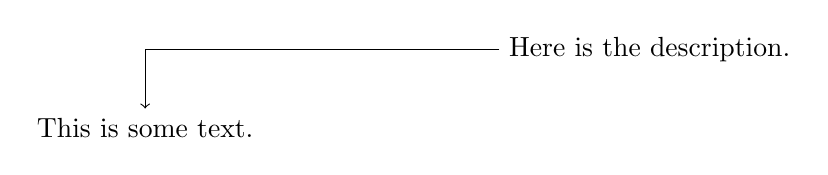
\begin{tikzpicture}
  \node[anchor=east] at (0,0) (text) {This is some text.};
  \node[anchor=west] at (3,1) (description) {Here is the description.};
  \draw[->] (description) -| (text);
\end{tikzpicture}


\begin{tikzpicture}
  \node[anchor=east] at (0,0) (text) {This is some text.};
  \node[anchor=west] at (3,1) (description) {Here is the description.};
  \draw[->] (description) .. controls ([xshift=-4cm] description) and ([xshift=4cm] text) .. (text);
\end{tikzpicture}


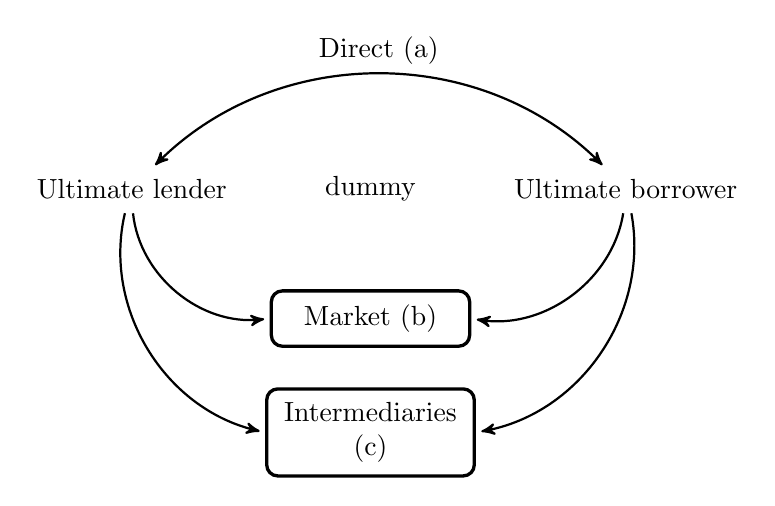
\begin{tikzpicture}[node distance=1cm, auto,]
\tikzset{
    %Define standard arrow tip
    >=stealth',
    %Define style for boxes
    punkt/.style={
           rectangle,
           rounded corners,
           draw=black, very thick,
           text width=6.5em,
           minimum height=2em,
           text centered},
    % Define arrow style
    pil/.style={
           ->,
           thick,
           shorten <=2pt,
           shorten >=2pt,}
}
 %nodes
 \node[punkt] (market) {Market (b)};
 \node[punkt, inner sep=5pt,below=0.5cm of market]
 (formidler) {Intermediaries (c)};
 % We make a dummy figure to make everything look nice.
 \node[above=of market] (dummy) {dummy};
 \node[right=of dummy] (t) {Ultimate borrower}
   edge[pil,bend left=45] (market.east) % edges are used to connect two nodes
   edge[pil, bend left=45] (formidler.east); % .east since we want
                                             % consistent style
 \node[left=of dummy] (g) {Ultimate lender}
   edge[pil, bend right=45] (market.west)
   edge[pil, bend right=45] (formidler.west)
   edge[pil,<->, bend left=45] node[auto] {Direct (a)} (t);
\end{tikzpicture}
\end{document}
